\chapter{Incertezza nelle decisioni mediche}
\label{cap:incertezza-decisioni-mediche}

% \intro{Brevissima introduzione al capitolo}\\

\section{Preambolo}
In quest'era di Medicina di Precisione e di Medicina predittiva, le incertezze che i medici devono affrontare sono sorprendentemente vaste, ben oltre le aspettative di una società che crede in una scienza moderna infallibile. Nonostante i progressi significativi nel campo della ricerca biomedica che promettono una precisione sempre maggiore nelle informazioni, i medici spesso si trovano a dover fare scelte basate su dati non completi e su una comprensione parziale di certe malattie. La medicina si trova a navigare in un mare di variabili aleatorie e incertezze, una realtà difficile da accettare per i pazienti, i quali cercano risposte chiare e sicure riguardo alla loro salute attuale e futura.
In sanità, l'incertezza non è un'eccezione ma una costante. Questa condizione viene descritta come l'incapacità di prendere decisioni a causa di una percezione soggettiva dell'ignoranza, definita come "meta-ignoranza". Spesso, l'ignoranza è considerata inaccettabile in ambito sanitario, che richiede certezze e prove inequivocabili per formulare previsioni accurate e decisioni professionali prive di dubbi. Di conseguenza, i professionisti sanitari possono sviluppare atteggiamenti di avversione o negazione dell'incertezza, cercando rifugio in false certezze.\\

Diviene quindi complesso per i medici comunicare queste sfumature, poiché potrebbe sembrare che ammettere la presenza di incertezza minacci la loro affidabilità. La responsabilità dei medici non è solo quella di gestire il rischio, ma anche di supportare i pazienti nel comprendere e accettare l'incertezza relativa alle loro condizioni cliniche. 
Un percorso diagnostico non è fatto da un'unica scelta, bensì è composto da una serie di scelte. C'è differenza tra la domanda da porsi per la terapia da seguire e quella da porsi nell'ambito delle diagnosi. Quando si tratta di scegliere la terapia del paziente infatti la domanda che ci si pone è: ““Se tratto un paziente con la tonsillite con l'antibiotico A, otterrò risultati migliori rispetto al placebo o all'antibiotico B?”. Invece nel caso del quesito diagnostico un esempio di domanda che ci si pone è:  “Qual è il migliore percorso che devo seguire per differenziare una tonsillite batterica, da trattare con antibiotico, da una faringite virale, da non trattare?”.
Nel caso più semplice in cui si hanno due esami da confrontare tra loro la risposta è immediata. Ma quando gli esami sono tanti e si vogliono confrontare percorsi più complessi allora aumenta l'incertezza. 
Le situazioni cliniche possono essere descritte come costituite da un nucleo di rischio, con probabilità di esito noto, circondato da una "nuvola" di incertezza, che diventa più ampia quanto più vaga e imprecisa è l'informazione clinica disponibile. Questa nuvola di incertezza deve essere sempre considerata, poiché influisce significativamente sulle probabilità degli esiti.
Hillen et al.\footcite{womak:tolleranza-incertezza} descrivono la tolleranza all'incertezza come una risposta comportamentale, cognitiva ed emotiva alla percezione soggettiva di ignoranza rispetto a una determinata situazione. Questa risposta può essere negativa, portando a dubbi, vulnerabilità e paura, o positiva, vedendo l'incertezza come un'opportunità accompagnata da serenità, coraggio, curiosità e speranza.


\section{Definizione}

Cosa si intende per incertezza? L'incertezza è un termine che assume diversi significati in vari ambiti del sapere. Etimologicamente, la parola certezza deriva dal verbo latino "cernere", che significa separare, distinguere. "Certum", il participio passato di "cernere", indica qualcosa di separato, distinto e chiaramente delimitato. Al contrario, le circostanze incerte sono quelle che non sono chiaramente distinguibili o separabili.\\

Non sorprende quindi che l'incertezza venga definita come incapacità di prendere decisioni. Questa incapacità può essere attribuita ai fatti e alla realtà o può riguardare il soggetto. Han et al. hanno definito l'incertezza come una "meta-ignoranza", ovvero la percezione soggettiva dell'ignoranza. In questa accezione, l'incertezza non è nella realtà, ma è un fenomeno cognitivo, emotivo e comportamentale che si manifesta nel soggetto incerto attraverso una serie di fenomeni cognitivi e affettivi, tra cui:

\begin{itemize}
    \item Dubbio;
    \item Percezione di indefinito;
    \item Percezione di indeterminazione;
    \item Sensazione di non essere credibili;
    \item Ansia;
    \item Comportamenti di evitamento dell'incertezza (ambiguity aversion);
\end{itemize}

Secondo Han et al identifichiamo almeno tre livelli di incertezza: \\
Il primo tipo di incertezza è quello scientifico, che deriva dalle informazioni con cui il professionista si confronta per prendere decisioni. L'incertezza è legata all'indeterminatezza degli eventi futuri, spesso espressa in termini percentuali di probabilità. Questa incertezza è misurabile e fornisce una guida utile per il decisore, ma non è eliminabile poiché rimane sempre una previsione probabilistica e non deterministica. Il grado di incertezza aumenta se le informazioni disponibili sono ambigue, ovvero non univoche, inaffidabili o difficili da interpretare. Cresce ulteriormente quando le informazioni sono complesse, con molteplici fattori causali, stati di eventi, esiti o interpretazioni possibili, e quando i confini tra eventi sono vaghi o difficili da descrivere.\\

Un secondo tipo di incertezza è di natura pratico-organizzativa, poiché qualsiasi intervento diagnostico o terapeutico dipende dalla qualità del sistema sanitario in cui è inserito. Infine, l'incertezza può derivare dalle informazioni fornite dal paziente stesso sulla propria salute e sulla sua rete di assistenza. Questo è particolarmente rilevante nelle cure primarie, dove quasi tutti gli interventi iniziano dalla soggettività del paziente.\\

Le situazioni cliniche possono quindi essere rappresentate come costituite da un nucleo di rischio noto, affrontabile con la conoscenza probabilistica, circondato da una nube di incertezza.\\


La fase di scelta terapeutica è particolarmente complicata. Esiste incertezza non solo sui dati oggettivi che dovrebbero guidare la selezione del trattamento più appropriato in termini di rischio e beneficio, ma anche sulla percezione soggettiva del paziente rispetto a queste scelte, e sul valore che attribuisce ai potenziali rischi e benefici. La decisione più efficace non emerge da un calcolo matematico delle probabilità di successo, ma è il risultato di una valutazione molto più complessa, basata sull'autonomia effettiva del paziente. 
Gli effetti dell'incertezza sono molteplici e possono essere psicologici per pazienti e medici, oltre che deontologici, etici e legali. L'incertezza incide sulla relazione medico-paziente e sugli aspetti organizzativi del sistema sanitario, sia a livello micro che macro, influenzando in particolare la qualità e l'appropriatezza delle cure.
L'incertezza è intrinseca alla pratica clinica e, sebbene la pandemia di COVID-19 l'abbia resa più evidente, essa è sempre esistita.\\

Negli ultimi sessant'anni, la capacità di diagnosi e trattamento ha subito una trasformazione radicale, così come il rapporto medico-paziente, con una crescente enfasi sull'autonomia del paziente, fondamentale per una pratica medica sia legale che etica. Questa evoluzione ha portato i pazienti a confrontarsi con decisioni spesso difficili, valutando i rischi e i benefici di una scelta terapeutica in base ai propri valori e necessità personali. Paradossalmente, i medici tendono a favorire la 'scelta' del paziente quando le prove sono incerte e i risultati poco chiari, ma sono più inclini a imporre le loro decisioni quando le evidenze supportano chiaramente una specifica opzione terapeutica.



\section{Nella pratica}
Nella pratica clinica, i medici si confrontano quotidianamente con informazioni probabilistiche per prendere decisioni. Esempi includono stime di sopravvivenza senza malattia in oncologia, valutazione del rischio cardiovascolare, e la probabilità di eziologia batterica o virale in infezioni respiratorie. L'incertezza che ne deriva è legata all'indeterminatezza degli eventi futuri, spesso espressa in percentuali di probabilità. Questa incertezza è misurabile e fornisce una guida utile al decisore, ma non è eliminabile, poiché rimane una previsione probabilistica e non deterministica.\\
Nelle situazioni più ambigue e con esiti incerti, è cruciale valutare attentamente il ruolo della consulenza medica nel supportare il processo decisionale. Le decisioni prese in assenza di dati affidabili sui benefici e i rischi delle diverse opzioni terapeutiche sono tra le più difficili e richiedono un maggiore coinvolgimento del medico. Se l'incertezza prevale e la scelta è complessa, non si può semplicemente lasciare la decisione al paziente, ma il medico deve assumersi la responsabilità professionale di guidare il processo decisionale.\\

L'incertezza decisionale può aumentare se le informazioni sono non solo probabilistiche ma anche ambigue. Un'informazione è ambigua quando è imprecisa (espressa come un ampio intervallo di valori), inaffidabile (derivata da strumenti o metodi non affidabili) o non univoca. Inoltre, l'incertezza aumenta ulteriormente se le informazioni sono complesse, cioè quando ci sono molteplici fattori causali, stati di eventi, esiti o interpretazioni possibili, e quando i confini tra eventi sono vaghi o difficili da descrivere.\\

Come spiegato nel libro \textit{L'arte della probabilità, certezze e incertezze nella medicina}\footcite{womak:arte-probabilita-coen}, di fronte all'incertezza, i medici tendono a consultarsi tra loro e utilizzano strumenti statistici per valutare il livello di concordanza. Uno di questi strumenti è l'indice K, che misura quanto due medici siano d'accordo nelle loro valutazioni. Se l'indice K è pari a 1, significa che c'è una concordanza totale, mentre un valore di 0 indica la massima discordanza. \\
In pratica, un indice K superiore a 0,61 indica un alto livello di concordanza tra i medici. Questo suggerisce che il risultato delle loro valutazioni sarà considerato più oggettivo quanto più i medici sono d'accordo nella loro interpretazione. Tuttavia, nella pratica quotidiana, raggiungere un indice K pari a 1 è molto raro, sia nella valutazione degli esami per immagini che nell'interpretazione dei segni clinici.

\section{Le euristiche e la valutazione del rischio}

Il ragionamento clinico è fondamentale in medicina per affrontare qualsiasi situazione. Oggi, si riconosce che l'approccio del medico alla situazione clinica non si basa solo su modelli analitici, consci e controllati dal ragionamento, ma anche su modelli non analitici, inconsci e intuitivi. L'insegnamento del metodo clinico raccomandato, quindi, include entrambe queste tipologie. Quando non è possibile affidarsi a un dato numerico o statistico i medici si affidano a quella che viene chiamata gut feeling, una sensazione di pancia, oppure all'euristica. \\
In queste occasioni è la sensazione del medico a indicare qual è la decisione giusta da prendere, c'è una sorta di consapevolezza fisica su quale sarebbe la decisione giusta, senza ragionarci troppo sopra. \\
Questa sensazione in realtà non è solo un'intuizione, è soprattutto un'attivazione del sistema nervoso enterico, che è composto da milioni di neuroni collegati al nostro intestino. \\
L'euristica somiglia al gut feeling perchè non è razionale. Si basa sull'identificazione di poche informazioni importanti, le valuta e interrompe la ricerca quando ritiene che queste informazioni siano sufficienti per una decisione adeguata 
La conclusione è che il percorso diagnostico del medico si alterna tra euristiche, ragionamento deduttivo, e confronto con altri. Tuttavia il processo decisionale è quasi sempre inconsapevole, sono pochissimi i medici che ragionano in termini numerici durante il loro processo diagnostico.
Un buon esempio di strategie decisionali rapide ma basate su evidenze sono le cosiddette clinical decision rules o clinical prediction rules, in cui pochi segni e sintomi, insieme a esami point-of-care, possono essere utilizzati per prendere rapidamente una decisione clinica. Allo stesso tempo, l'euristica viene spesso utilizzata dai medici senza l'aiuto statistico, per prendere decisioni in situazioni incerte, considerando anche elementi di contesto secondo i principi della razionalità ecologica.\\

Gigerenzer dimostra come nelle situazioni di rischio conosciuto, i sistemi di decisione basati sull'analisi delle probabilità siano i migliori, mentre nelle situazioni di incertezza, le strategie euristiche rapide dei professionisti abbiano maggiore successo. In medicina, quindi, in molti casi, le strategie rapide possono essere più efficaci di quelle basate esclusivamente su metodi analitici. Utilizzare strategie euristiche evita anche di aumentare le indagini diagnostiche in situazioni di incertezza.\\

La valutazione del rischio è un altro aspetto cruciale nell'ambito delle incertezze. In molte situazioni è possibile conoscere rischi e benefici di un'operazione o gli esiti di un trattamento, ma quando entra in gioco l'ambito dell'incertezza diventa più difficile stimare i rischi. \\
Ad oggi poco più del 20\% delle indicazioni delle linee guida ha una valutazione di tipo 1A (ovvero elevato grado di documentazione clinica e alto livello di raccomandazione). Tutto il resto delle indicazioni si basa su un largo consenso riscosso, più che di numeri che provano l'effettiva bontà delle soluzioni proposte. 


\section{Rapporto con il paziente}

Comunicare le incertezze al paziente è fondamentale per costruire un percorso decisionale consapevole. Nonostante la medicina moderna si basi su numeri e analisi statistiche di  esperienze pregresse, presupponendo che ogni opzione diagnostica o terapeutica sia la più appropriata, la comunicazione del medico trasmette non solo logica, ma anche significato, influenzando la percezione del paziente e le sue aspettative. È essenziale che la comunicazione delle incertezze non confonda ulteriormente il paziente, ma che si adatti alle sue caratteristiche individuali (età, cultura, fattori psicologici) sia nella complessità dell'informazione che nel linguaggio utilizzato. È certo però che dal punto di vista del paziente l'ignoranza dei medici riguardo queste aree di incertezza può indurre una diffidenza che non aiuta la comunicazione tra le parti. \\
L'incertezza può essere percepita come alta o bassa, a seconda delle misurazioni dei vari aspetti sopra descritti. Questo grado di incertezza è fondamentale per scegliere la strategia clinica e comunicativa. I professionisti sanitari valutano la gravità della situazione e della patologia, il rischio di un esito negativo se gli interventi vengono omessi, e il rischio degli interventi stessi, basandosi su misure di probabilità.\\

\begin{figure}[!ht] 
    \centering 
    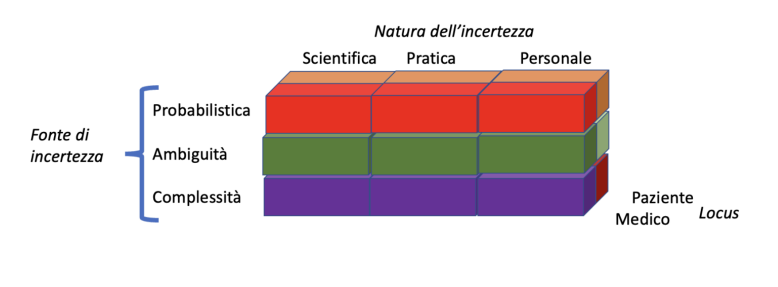
\includegraphics[width=0.9\columnwidth]{fonti-incertezza} 
    \caption{Natura dell'incertezza}
\end{figure}

Le situazioni cliniche possono essere rappresentate come costituite da un nucleo di rischio conosciuto, affrontabile con la conoscenza probabilistica, circondato da una nube di incertezza. La gestione dell'incertezza in medicina non dovrebbe limitarsi a una semplice ricognizione anamnestica, ma deve essere un aspetto chiave del metodo clinico, incorporato in tutti gli aspetti del processo decisionale dei professionisti sanitari. Questo è essenziale per attuare azioni appropriate.\\
\begin{figure}[!ht] 
    \centering 
    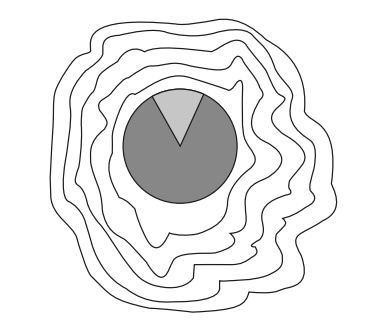
\includegraphics[width=0.9\columnwidth]{incertezza-situazioni-cliniche} 
    \caption{Illustrazione di come si presentano le situazioni cliniche}
\end{figure}


Nel processo decisionale clinico, l'incertezza influisce sulla probabilità che un evento si verifichi o meno. Riconoscere l'incertezza consente di comunicarla, prendere decisioni più consapevoli e praticare una medicina più prudente e meno onnipotente.
In base alle preferenze espresse dal paziente, possiamo costruire una rete protettiva (safety net) adottando una strategia di attesa. Prescriviamo un sintomatico e informiamo il paziente in modo strutturato sui sintomi di allarme (red flags) che potrebbero presentarsi, nonché sui tempi e le modalità per cercare aiuto medico se questi sintomi si manifestassero o se non ci fossero miglioramenti in un periodo prestabilito. Idealmente, queste informazioni dovrebbero essere fornite per iscritto, dopo un processo decisionale condiviso.\\

Esistono situazioni in cui la diagnosi è incerta e l'alternativa potrebbe essere una malattia grave a progressione rapida. In questi casi, si può utilizzare il tempo come un test, simile a un esame ematico o strumentale. L'aspetto comunicativo della strategia è cruciale. Il medico deve creare una buona relazione di fiducia e collaborazione con il paziente, affinché quest'ultimo possa comprendere chiaramente le istruzioni. Il paziente deve essere consapevole dell'incertezza diagnostica, dei segni e sintomi a cui prestare attenzione e del periodo di osservazione, nonché sapere come cercare aiuto.\\

È fondamentale anche l'aspetto organizzativo: il medico e il suo team devono avere accesso alle informazioni sulla decisione presa con il paziente in ogni momento, e deve esistere un sistema di ricezione delle chiamate che preveda una risposta immediata.\\

In generale, i risultati non sono sempre chiari, quindi gli autori invitano i medici alla prudenza, a utilizzare la rete protettiva e a insegnarla nel training della medicina generale, in attesa di maggiori risultati sull'efficacia di questa pratica. Tuttavia, lo strumento più potente per aiutare il medico a decidere nell'incertezza è la condivisione del processo decisionale con il paziente o con chi se ne prende cura.\\

In che modo il contributo del paziente può influire sul processo decisionale in medicina? Kon sostiene che la decisione condivisa esiste su un continuum con il modello paternalistico (guidato dal medico) a un'estremità e il modello informativo (guidato dal paziente) all'altra, mentre al centro c'è la \textit{decisione condivisa}\footcite{womak:decisione-condivisa-kon} in cui medico e paziente contribuiscono equamente, ciascuno al 50\%.\\


\begin{figure}[!ht] 
    \centering 
    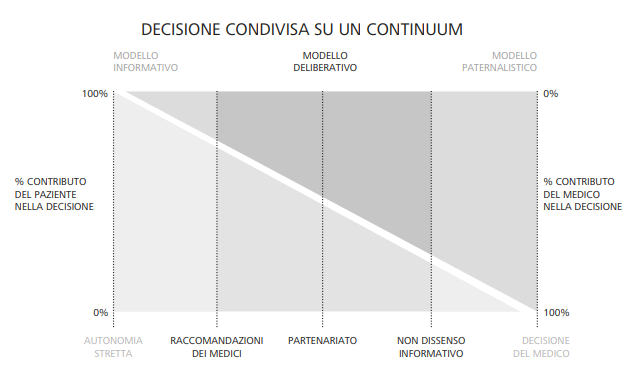
\includegraphics[width=0.9\columnwidth]{decisione-condivisa-kon} 
    \caption{Modello della decisione condivisa secondo Kon}
\end{figure}

Occorre considerare quale situazione clinica richiede un maggiore coinvolgimento del paziente. Questa è spesso una situazione di incertezza, contrapposta a una in cui esiste una chiara opzione migliore con un rapporto costi/benefici ben definito. In contesti incerti, le preferenze e i valori del paziente diventano cruciali poiché non ci sono rapporti chiari tra costi e benefici. Più è grande l'incertezza, più è necessario coinvolgere il paziente, valutando le sue conoscenze e capacità. Questo non significa solo considerare le preferenze, ma anche integrare il contributo del paziente nella decisione.\\

È importante distinguere la decisione condivisa dal semplice consenso informato. Quest'ultimo implica un flusso informativo unidirezionale dal medico al paziente, che è eticamente e legalmente obbligatorio ma non necessariamente parte di una decisione già presa dal medico. La vera decisione condivisa implica invece uno scambio di idee tra medico e paziente, una collaborazione che porta a una decisione comune. In questo processo, il paziente agisce come consulente, aiutando il medico a prendere una decisione, il che è molto diverso da un semplice processo informativo.


\section{Guida nell'analisi dell'incertezza secondo l'EFSA}
Il comitato scientifico dell'Autorità europea per la sicurezza alimentare (EFSA) ha sviluppato una guida dettagliata\footcite{womak:guida-analisi-incertezza} sull'analisi dell'incertezza nelle valutazioni scientifiche, con l'obiettivo di fornire una base solida per il processo decisionale in situazioni di incertezza.\\

Il comitato scientifico dell'EFSA è composto da eminenti scienziati di tutta Europa, ciascuno con una comprovata eccellenza scientifica e una vasta esperienza in varie discipline rilevanti per il mandato dell'EFSA. Tra le loro competenze si annoverano la valutazione dei rischi per la salute umana, l'epidemiologia, la microbiologia, la nutrizione umana, la chimica, la biologia e molte altre aree scientifiche. Questo gruppo multidisciplinare lavora per sviluppare metodologie armonizzate di valutazione del rischio e per garantire l'omogeneità dei pareri scientifici.\\

Le questioni affrontate dal comitato sono spesso di natura multidisciplinare, richiedendo approcci innovativi e integrati per la valutazione del rischio. Tra queste, vi sono l'armonizzazione dell'uso di ipotesi predefinite in assenza di dati reali.\\

Secondo tale comitato, l'analisi dell'incertezza nelle valutazioni scientifiche varia a seconda della natura della valutazione stessa. È essenziale identificare il tipo di valutazione in corso per poi seguire le linee guida specifiche.\\

Tipologie di Valutazione:
\begin{itemize}
    \item Valutazioni Standardizzate: Queste seguono procedure prestabilite e dettagliate, spesso utilizzate per prodotti regolamentati come le autorizzazioni di preimmissione sul mercato. Queste procedure richiedono dati da studi specifici e includono criteri e calcoli standardizzati.
    \item  Valutazioni Specifiche per il Caso in Esame: Necessarie quando non esistono procedure standardizzate. I valutatori devono sviluppare un piano di valutazione personalizzato, utilizzando elementi standardizzati dove possibile ma adottando approcci specifici per altre parti.
    \item  Elaborazione o Revisione di Documenti Orientativi: Coinvolge la creazione o l'aggiornamento di procedure standardizzate.
    \item  Valutazioni Urgenti: Richiedono completamento rapido con risorse limitate e implicano approcci semplificati.
    
\end{itemize}

In alcune aree dell'EFSA, una valutazione standardizzata può evidenziare la necessità di un'analisi più approfondita. In questi casi, si passa a una valutazione specifica per il caso, sostituendo elementi standardizzati con approcci su misura.
Le valutazioni possono essere quantitative (stima di una quantità) o qualitative (risposta verbale a una domanda). Anche se una valutazione è qualitativa, le conclusioni devono essere ben definite. L'incertezza può essere espressa quantitativamente tramite probabilità, pertanto, è raccomandato che i valutatori cerchino di quantificare l'incertezza anche quando utilizzano metodi qualitativi, poiché i metodi qualitativi hanno comunque un ruolo importante nell'analisi dell'incertezza.\\

\subsection{Analisi dell'incertezza per le valutazioni standardizzate}
Quando si analizza l'incertezza in una valutazione standardizzata, è cruciale distinguere tra incertezze standard e non standard. Prima di tutto, bisogna determinare se esistono incertezze non standard. Se non ci sono, basta riportare che la valutazione non presenta incertezze non standard. In caso contrario, bisogna valutare l'impatto di queste incertezze sul risultato della procedura standard. Se l'incertezza non standard è significativa, potrebbe essere necessario passare a una valutazione specifica per il caso in esame.\\

\subsection{Analisi dell'incertezza per valutazioni specifiche per il caso in esame}

Per le valutazioni specifiche per il caso, i valutatori devono seguire istruzioni pertinenti e, se necessario, consultare pareri scientifici di supporto. Dopo aver pianificato la valutazione e identificato le incertezze, bisogna decidere se suddividere l'analisi dell'incertezza in parti. Questa scelta dipende dalle domande e quantità rilevanti per la valutazione. \\
Valutare le incertezze collettivamente è il metodo più semplice, dove tutte le incertezze vengono valutate insieme nell'ambito della valutazione specifica.

Se l'analisi richiede risposte a domande sì/no, i valutatori possono esprimere le incertezze utilizzando probabilità e combinarle tramite calcoli. Questo richiede che ogni parte dell'analisi risponda a domande sì/no e che il ragionamento sia espresso in un modello logico formale. In alternativa, le incertezze possono essere valutate separatamente, sia qualitativamente che quantitativamente, e poi combinate secondo giudizio esperto. Anche se alcune parti vengono valutate qualitativamente, è consigliabile esprimere un giudizio di probabilità per la valutazione complessiva.\\

In caso di valutazioni scientifiche urgenti, i valutatori devono adottare un approccio rapido che si adatti ai tempi e alle risorse disponibili. Anche in situazioni di emergenza, l'analisi dell'incertezza è essenziale. Pertanto, si consiglia di valutare tutte le incertezze in un unico passaggio. Questo metodo, sebbene meno preciso rispetto ad altri, offre una base ragionevole per una consulenza preliminare, a condizione che l'incertezza aggiuntiva della valutazione semplificata sia chiaramente indicata nelle conclusioni.\\

Durante la creazione o la revisione di documenti di orientamento contenenti procedure standardizzate, è spesso necessario eseguire un'analisi dell'incertezza. Questa analisi verifica se la procedura proposta è sufficientemente prudenziale e se soddisfa gli obiettivi di gestione per quella specifica classe di prodotti o problemi. Una procedura ben calibrata può essere applicata ripetutamente senza dover valutare le incertezze standard ogni volta.\\

Se un'analisi dell'incertezza è richiesta per altri motivi durante lo sviluppo di un documento di orientamento, essa deve essere trattata come una valutazione specifica per il caso in esame. Quando una procedura viene utilizzata in più aree di lavoro dell'EFSA, la sua calibrazione e revisione devono essere svolte congiuntamente da tutti i soggetti coinvolti. Inoltre, se una procedura standardizzata fa parte di un protocollo internazionale, eventuali modifiche devono essere apportate in consultazione con i partner internazionali e la comunità scientifica.\\

\subsection{Individuazione delle incertezze}

\subsubsection{Incertezze standard e non standard}

Incertezze standard: Sono gestite da procedure standardizzate o da elementi standardizzati della valutazione. Ad esempio, nella valutazione del rischio chimico, un fattore di default pari a 100 può gestire le incertezze relative alla tossicità. In studi sperimentali, l'incertezza di misurazione è considerata standard se le linee guida sono state seguite senza deviazioni. Le incertezze standard non devono essere riconsiderate in ogni nuova valutazione che segue la procedura standard, poiché sono già state valutate durante la definizione della procedura stessa.\\

Incertezze non standard: Includono qualsiasi deviazione da una procedura standard o elementi non coperti dalla stessa. Ad esempio, studi che non seguono le linee guida standard o che presentano carenze nella reportistica, oppure l'uso di studi non standard o di "livello superiore". Queste incertezze devono essere valutate caso per caso, poiché non sono coperte dal margine di manovra delle incertezze standard.\\

Proporzione delle incertezze: In ogni tipo di valutazione possono esserci sia incertezze standard che non standard, ma in proporzioni variabili. Le valutazioni standardizzate tendono ad avere meno incertezze non standard, mentre altre valutazioni ne presentano di più.



\subsection{Procedure per l'individuazione delle incertezze} 

\textbf{Fonti di incertezza:} Ogni valutazione deve indicare le fonti di incertezza individuate, preferibilmente sotto forma di elenco o tabella, per trasparenza.

\textbf{Verifica sistematica:} I valutatori devono verificare sistematicamente le incertezze in ogni parte della valutazione, includendo sia gli input (dati, stime, evidenze) che i metodi utilizzati (metodi, calcoli, modelli statistici, ragionamento, giudizio esperto), per ridurre al minimo il rischio di tralasciare incertezze importanti. Nelle valutazioni standardizzate, devono essere individuate solo le incertezze non standard.

\textbf{Incertezze negli input:} Queste vengono individuate durante la valutazione delle evidenze dalla letteratura o dai database esistenti. Se sono disponibili approcci strutturati per la valutazione delle evidenze, dovrebbero essere utilizzati. Altrimenti, i valutatori possono usare la Tabella 1 come guida per individuare le incertezze negli input. Devono anche prestare attenzione a eventuali incertezze aggiuntive non elencate.

\textbf{Incertezze nei metodi}: Queste non sono generalmente gestite dagli schemi di valutazione delle evidenze esistenti. I valutatori dovrebbero utilizzare la colonna destra della Tabella 1 per individuare le incertezze nei metodi applicati alla valutazione. Anche qui, devono essere considerati eventuali tipi aggiuntivi di incertezza.

\textbf{Uso delle tabelle:} Le tabelle e gli elenchi devono facilitare l'individuazione delle incertezze, non la loro classificazione. I valutatori non dovrebbero impiegare troppo tempo a far corrispondere le incertezze alle tipologie elencate.

\textbf{Classificazione delle incertezze:} I valutatori devono determinare quali incertezze sono standard e quali non lo sono, poiché questo influenzerà come verranno gestite nei passaggi successivi dell'analisi dell'incertezza.

\begin{figure}[!ht] 
    \centering 
    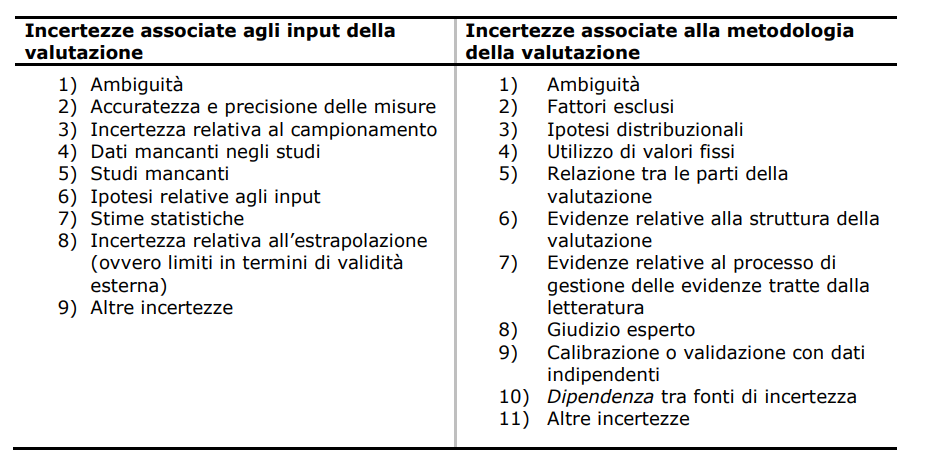
\includegraphics[width=0.9\columnwidth]{tipologia-incertezze} 
    \caption{Natura dell'incertezza}
\end{figure}

\subsubsection{Definizione delle priorità delle incertezze}

Definire le priorità delle fonti di incertezza è utile in diverse fasi della valutazione. All'inizio, aiuta a selezionare le incertezze più importanti per un'analisi approfondita. Durante la valutazione, individua le aree in cui cercare più dati o coinvolgere ulteriori esperti. Alla fine, identifica potenziali aree di ricerca futura. Le priorità dovrebbero basarsi sul contributo di ciascuna fonte di incertezza all'incertezza complessiva della valutazione, tenendo conto della dimensione dell'incertezza e della sua influenza sul risultato.
L'influenza delle diverse incertezze può essere valutata utilizzando giudizi esperti e scale ordinali. Si possono utilizzare metodi come le “tabelle d'incertezza” o l'approccio NUSAP.

Quando si usano modelli quantitativi, l'analisi di sensibilità può valutare l'influenza delle incertezze sugli input del modello. Le scelte riguardanti la struttura del modello possono essere verificate ripetendo la valutazione con alternative.

Per affrontare l'incertezza in modo efficace, è fondamentale che la valutazione sia suddivisa in parti principali, come esposizione e pericoli in una valutazione del rischio chimico, e in parti minori, come singoli parametri o studi. Questa suddivisione consente di eseguire l'analisi dell'incertezza a diversi livelli: valutare tutte le incertezze collettivamente, suddividerle in parti principali e combinarle successivamente, o suddividerle ulteriormente in parti più piccole e combinarle gradualmente. È essenziale combinare le parti dell'analisi per caratterizzare l'incertezza complessiva, definendo in anticipo come queste parti verranno integrate. Utilizzare un diagramma di modello concettuale può migliorare la trasparenza e il rigore del processo.\\

L'efficienza e l'affidabilità della valutazione dipendono dal livello di suddivisione scelto. Trattare separatamente le parti con incertezze rilevanti è generalmente più affidabile, mentre valutare tutte le incertezze collettivamente può essere più rapido ma meno preciso. Alcune incertezze minori possono essere considerate in una fase successiva della caratterizzazione complessiva, mentre quelle maggiori dovrebbero essere combinate tramite calcoli per garantire maggiore affidabilità. Quando si utilizzano modelli quantitativi, è utile quantificare l'incertezza per ciascun parametro e considerare anche le incertezze non quantificate, come quelle relative alla struttura del modello.\\

Per valutare correttamente l'incertezza, è essenziale che le domande e le quantità d'interesse siano chiaramente definite. Qualsiasi ambiguità aggiunge ulteriore incertezza e complica la valutazione. Se una domanda o quantità non è già ben definita, i valutatori devono provvedere a farlo per l'analisi dell'incertezza. Una quantità o domanda è ben definita se i valutatori possono concordare sulla risposta. Per ottenere ciò, si può specificare un esperimento, uno studio o una procedura che determinerebbe la risposta. Ad esempio, una misura ben definita per una quantità d'interesse dovrebbe includere specifiche di tempo, popolazione, luogo e condizioni. Allo stesso modo, la presenza o assenza di condizioni o meccanismi specifici deve essere dettagliata, così come i risultati di uno studio scientifico o un calcolo rilevante per la valutazione. Durante la formulazione delle domande, è importante identificare e sostituire termini ambigui o soggetti a giudizio di gestione del rischio con termini più chiari o numeri. Se i termini di riferimento sono aperti, è necessario che le conclusioni siano riferite a quantità ben definite o contengano affermazioni chiare e ben definite, necessarie per valutare ed esprimere l'incertezza associata.\\

L'espressione qualitativa dell'incertezza utilizza parole o categorie ordinali, senza quantificare le possibili risposte o probabilità. Questo metodo è utile in varie situazioni, come la definizione delle priorità delle incertezze e la descrizione di singole fonti di incertezza durante l'analisi. Le espressioni qualitative sono utili per definire le priorità, descrivere singole fonti di incertezza come passaggio preliminare per la quantificazione complessiva, comunicare i risultati usando una scala di probabilità approssimata con descrittori qualitativi, descrivere incertezze non incluse nella valutazione quantitativa e per la reportistica quando richiesto da decisori o normative.\\

Per descrivere singole fonti di incertezza, si raccomanda l'uso di scale ordinali per migliorare coerenza e trasparenza. Queste scale dovrebbero essere parte della pianificazione della valutazione e possono variare in formalità a seconda delle necessità. Le espressioni qualitative dovrebbero essere usate per elaborare un giudizio quantitativo sull'impatto combinato delle incertezze, basandosi su una logica chiara e non su calcoli arbitrari.\\

\subsection{Quantificare l'incertezza tramite probabilità}

Il Comitato scientifico raccomanda di esprimere quantitativamente l'impatto combinato delle incertezze. Le probabilità, specificate completamente o parzialmente, possono essere derivate da dati o giudizio esperto.\\

\textbf{Probabilità:} La probabilità varia da 0 a 1, espressa come percentuale da 0\% a 100\%. Per una domanda sì/no, 0\% significa che la risposta è sicuramente negativa, 100\% che è sicuramente positiva, e valori intermedi rappresentano vari gradi di certezza.\\

\textbf{Distribuzioni di probabilità:} L'incertezza relativa a una quantità non variabile può essere espressa tramite una distribuzione di probabilità, mostrando la probabilità relativa di diversi valori. Un'espressione parziale dell'incertezza può indicare la probabilità che un intervallo di valori includa il valore reale.\\

\textbf{Uso dei dati:} Quando disponibili, i dati dovrebbero essere utilizzati tramite analisi statistica, anche se il giudizio esperto interviene sempre, ad esempio nella scelta del modello  statistico. L'incertezza può essere quantificata direttamente o tramite calcoli dopo aver quantificato singole fonti di incertezza.\\
